\documentclass[a4paper,12pt]{report}
\usepackage[left=2.5cm,right=2.5cm,top=2.5cm,bottom=2.5cm]{geometry}
\usepackage{amsfonts}
\usepackage{graphicx}
\usepackage{hhline}
\usepackage{hyperref}
\usepackage{float}
\bibliographystyle{apalike}

\makeatletter
\renewcommand*\l@section{\@dottedtocline{1}{1.5em}{2.3em}}
\makeatother

\makeatletter
\def\@seccntformat#1{%
  \expandafter\ifx\csname c@#1\endcsname\c@section\else
  \csname the#1\endcsname\quad
  \fi}
\makeatother

\makeatletter
\let\latexl@section\l@section
\def\l@section#1#2{\begingroup\let\numberline\@gobble\latexl@section{#1}{#2}\endgroup}
\makeatother


\hypersetup{
    colorlinks=true,
    linkcolor=blue,
    filecolor=blue,      
    urlcolor=blue,
    citecolor=blue
}
\usepackage{caption}
\captionsetup[figure]{labelfont={color=blue, it}, font={footnotesize, color=black} }


\usepackage{titling}
\renewcommand\maketitlehooka{\null\mbox{}\vfill}
\renewcommand\maketitlehookd{\vfill\null}
\begin{titlepage}
\title{{PhD Thesis Synopsis}\\{\vspace{-0.29em} \hrulefill\\} \textbf{Microscopy and image analysis based enhancements for investigating DNA damage responses in cells}}
\author{P S Kesavan\\ {\vspace{6em}(Under the supervision of Prof. Aprotim Mazumder)}}
\date{}
\end{titlepage}

\linespread{1.5}
\begin{document}

\maketitle
\newpage
\tableofcontents
\newpage

\chapter{Introduction}
\section{DNA damage responses in cells}
Living organisms are continuously subjected to external and internal conditions that cause damage to their genetic material. It is estimated that a single mammalian cell is susceptible to upto 100,000 damaging events in a day \cite{ciccia2010dna}. When left unrepaired, such damages can result in mutations that can give rise to the downstream development of different cancers, and neurodegenerative diseases \cite{friedberg2005dna}. To overcome this problem of damage and error propagation in genetic information, cells have evolved diverse error detection and correction mechanisms, collectively known as DNA damage responses (DDR) \cite{hoeijmakers2009dna}. DDR often utilizes post-translational modifications (PTM), such as ubiqutination, phosphorylation, methylation etc. to propagate damage signals to downstream transducer proteins, like ATM or ATR. These transducers further effect higher-level decisions, such as checkpoint arrest to give the cell more time to repair, or if the damage is too extensive, proceed to apoptosis \cite{derks2014dna}.

\subsection{Features of DNA}
\paragraph*{} All known life on Earth stores their hereditary information in deoxyribose nucleic acid (DNA), a molecule that can be chacterised as a continous, unbranched linear chain, which is paired to a complementary strand to make the double helix. DNA is made of a deoxyribose sugar with a phosphate group between sugars, and to each sugar is attached a nitrogenous base. The combination of the sugar, phosphate group and the nitrogenous base is known as the nucleotide. There are four nitrogenous bases commonly found in DNA, which are Adenine (A), Guanine (G), Thymine (T) or Cytosine (C). The bases in opposite strands of DNA are complimentary in nature, with A pairing opposite T, and G pairing opposite C which allows for data redundancy at the encoding level on the storage medium. 

\paragraph*{} Much of the chemically encoded information of the genetic material is thought to be in the storage of the synthesis sequence of a polypeptide chain by ribosomes. In the coding sequence of the DNA, a unit of three nucleotide (called codons) is known to be encoding an amino acid. This is established as the genetic code, with a combination of 64 three letter nucleotide sequence coding for 20 different amino acids commonly found in the proteins. There are start and stop codons that define the boundary of coding sequence in the linear chain of DNA. Since there are more codons than amino acid, more than a single codon can encode for an amino acid. For instance, for Lysine, the three-letter codes are AAA and AAG.

\paragraph*{} DNA, because of its chemical nature, has a tendency to react with the chemical environment that surrounds it. This makes the information stored in this molecule to become inherently unstable over time, as the chemical environment can gradually change the molecule in different ways. Largely, chemical reactions can affect the genetic material in the level of the nitrogenous base, the nucleotide, and the phosphodiester bond. The base can be subjected to damages due to spontaneous processes such as deamination, or methylation. There can also be oxidative damage to the amino groups due the prescence of free radicals.


\subsection{Sources of damage}
\paragraph*{} For convinience, the sources of damage can be largely grouped as factors outside the cell, or exogenous sources, and factors inside the cell, arising from the overall cellular machinery, which are endogenous to the cells. Exogenous sources may include ionizing radiations from space, high energy photons from Sun, or carcinogenic industrial chemicals that are present in the environment due to human activity. Endogenously, chemical biproducts in biogenesis results in the formation of free radicals, which when in proximity to another molecule can freely exchange electrons, changing the electronic configurations of molecules, creating unstability.

\paragraph*{} CPD, UV products, etc.

\subsection{DNA repair}
\paragraph*{} DNA that is damaged has to be repaired. Since there are several types of damage that are chemically distinct, it is not surprising that natural selection has evolved a series of mechanisms to sense and repair damage. Also, unlike other DNA processes, such as replication or transcription, damages to DNA are stochastic, which requires repair systems to have a close watch on the molecular health of the DNA. The repair mechanism is an event based system that triggered by a chemical damage event. This further triggers downstream recruitment of repair factors to the site of damage.

\subsection{Chromatin in DDR}
\paragraph*{} In eukaryotes, DNA is packaged as chromatin with the help of nucleosomes. In-vitro experiments have shown that the presence of nucleosomes hampers repair processes such as base excision repair (BER) and nucleotide excision repair (NER) \cite{hara2000dna, odell2011nucleosome}. This further increases the complexity of our understanding of DDR, as the repair processes have to seamlessly operate within the context of chromatin, which is a refractory environment for repair. However, chromatin modifying factors, such as SWI/SNF, histone acetyletransferases (HATs) have been shown to be recruited to sites of damage \cite{park2006mammalian, polo2010regulation}. Chromatin integrity factor, KAP-1, has been found to be a substrate of ATM, which shows chromatin modulation can be a downstream transducer effect of DDR \cite{ziv2006chromatin}. These results indicate that there exists an interplay between chromatin and DDR, which have traditionally been seen as distinct fields of study.

\paragraph*{} It has been shown that damage repair characteristics vary across the nucleus depending on the density of chromatin packaging. Markers of damage are seen to persist for longer in sites of densely packed DNA (heterochromatin regions) as compared to sites of loosely packed DNA (euchromatin regions) \cite{goodarzi2008atm}.

\paragraph*{} Since DDR processes and their complex boundaries with other known and unknown biological systems are not well-understood, it presents an opportunity to develop tools and techniques from across the fields of microscopy, robotics and image processing to study such biological processes in scale. While there have been studies of DDR in living cells using tools of live cell microscopy, these have used indirect readouts of chromatin compaction states and also have been limited in terms of throughput. Progress towards uncovering DDR would immensely help in addressing fundamental problems related to biological circuitry, such as stochasticity in responses, and further our knowledge of disease biology.

\subsection{Methods to study DDR in chromatin}
\paragraph*{} To this end in this thesis, I first describe the development of fluorescence anisotropy imaging tools to investigate chromatin compaction states upon laser-induced double strand breaks. Further to improve the throughput of such microscopic investigations we develop methods that improve statistics in both fixed and live cell investigations of DDR.



DNA in the eukaryotic cell nucleus is packaged into chromatin with histones and other protein components. This genetic material is susceptible to damage from different sources. It is estimated that in a day, a single mammalian cell can face as many as 100,000 lesions to its DNA (Ciccia and Elledge, 2010). If left unrepaired, such damage can result in cell cycle arrest, cell death, or senescence, or, at the level of the organism, cause mutations that result in diseases such as cancers or neurodegenerative diseases (Friedberg et al., 2006; Madabhushi et al., 2014). To deal with this constant assault on genetic material, cells have evolved a cohort of mechanisms that sense and repair DNA damage (Hoeijmakers, 2009).

Every DNA damage response (DDR) in eukaryotic cells takes place in the context of chromatin. Biochemical studies in in vitro systems with synthetically damaged DNA have helped uncover the critical role that chromatinization plays in DDR. In experiments with purified systems of repair, when a nucleosome was added to the naked DNA, measurements of repair kinetics by nucleotide excision repair (NER) and base excision repair (BER) indicated that the repair was much slower than that of naked DNA without a nucleosome (Hara et al., 2000; Odell et al., 2011). This led to the conclusion that the proteins that help package DNA inside the nucleus can have a hindering effect on damage repair. In cells, regions undergoing repair have been found to be more sensitive to micrococcal nuclease digestion than bulk DNA (Smerdon et al., 1978). This indicates that DNA can be more exposed during damage repair. Proteins that modify nucleosomes, such as SWI/SNF, and histone acetyltransferases (HATs), such as CHD4, have been found to be recruited to the site of damage, which indicates that the chromatin at the site of damage may be relaxed as a response to damage (Park et al., 2006; Polo et al. 2010). Further proteins that maintain chromatin integrity, such as KAP-1, have been found to be substrates for the DDR master kinase, ATM (Ziv et al., 2006).

A previous study has found that markers of repair persist in heterochromatin regions for longer time than in euchromatic regions (Goodarzi et al., 2008), indicating that the dynamics of repair is sensitive to the compaction state and activity of chromatin. With core histone H2B tagged with GFP and microirradiation of Hoechst-sensitized cells, it has been shown that chromatin is decompacted at the site of damage in response to clustered double-strand breaks (DSBs), followed by a phase of increased compaction (Kruhlak et al., 2006; Strickfaden et al., 2016). Compaction of chromatin is critical to DDR, and compaction in the absence of damage is sufficient to stimulate a damage response, independent of damage (Burgess et al., 2014). However, in experiments using microscopy, the spreading or shrinking of a chromatin region marked with a specific fluorescent histone has been used as a proxy for chromatin compaction, and as such does not report directly on physical state of the chromatin. In other studies, fluorescence anisotropy imaging (FAI) has been used to map the compaction of chromatin in living cells directly (Banerjee et al., 2006). Core histone H2B tagged with EGFP is excited with polarized light, which preferentially excites EGFP molecules whose excitation dipoles are oriented along the polarization axis of the excitation light. The extent of depolarization of the emission light gives a measure of the rotational diffusion of EGFP fusion proteins. The higher the rotational diffusion, the greater is the extent of depolarization of the emission signal, over and above what would be expected because of random orientations of the fluorophores. Fluorescence anisotropy is a measure of the extent of depolarization (Lakowicz, 2006; Ghosh et al., 2012). Since H2B-EGFP in the regions of euchromatin should have greater rotational mobility than regions of heterochromatin, anisotropy maps generated by FAI show evidence of differential compaction of chromatin and as such could be used as a direct physical measure of local chromatin packaging (Bhattacharya et al., 2009; Makhija et al., 2014). In this study, we sought to use FAI in the context of DDR to monitor chromatin compaction states directly. Chromatin decompaction is essential for repair, and yet local chromatin compaction may be used by cells to prevent further damage (Burgess et al., 2014). Using FAI, we studied the physical changes to the chromatin structure in response to laser microirradiation–induced clustered DSB, in regions of chromatin beyond just the site of damage. We show that anisotropy maps are preserved in fixation and regions of high and low anisotropy indeed correspond to physiologically relevant markers for heterochromatin and euchromatin, respectively. This also allows us to first follow compaction changes in response to localized DSBs in living cells, and then fix the cells and perform immunofluorescence for markers of DNA damage. Finally, we follow the differential dynamics of two endogenous damage-responsive proteins (PCNA and PARP1) with respect to chromatin compaction maps and show that their time scales of recruitment and subsequent dispersion are very different. In addition to being recruited at the site of damage, PCNA also forms nodes further away in regions of low anisotropy. These PCNA nodes in open chromatin incorporate deoxynucleotide analogs, indicating that individual DSBs from the laser-induced cluster may be extruded out from the site of damage for the purposes of repair. Together, these studies open up a new avenue of following DDR in live cells in the chromatin, while also taking advantage of different immunofluorescent markers for DNA damage and chromatin.
\chapter{Fluorescence Anisotropy Imaging for assaying chromatin compaction states in live cells}
\begin{figure}[!htp]
    {\hfill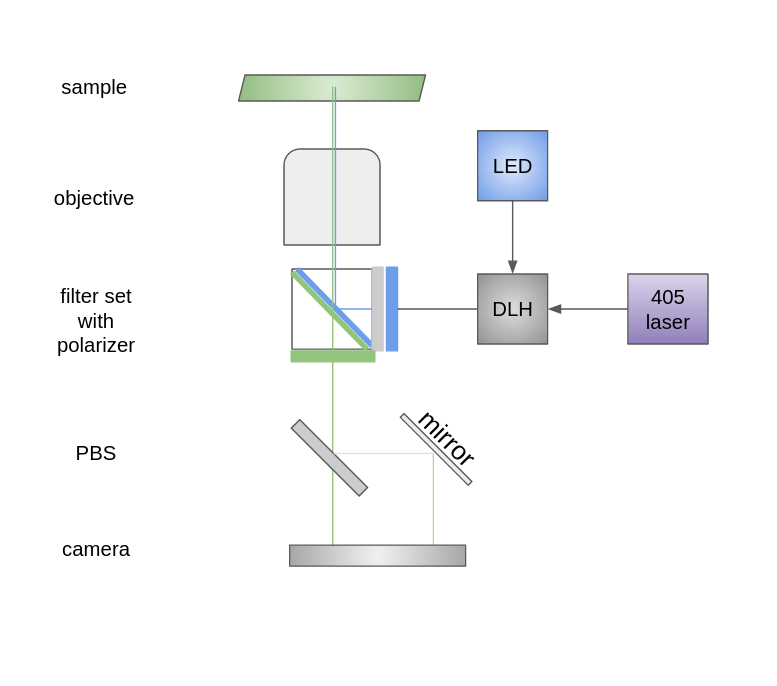
\includegraphics[trim=0 50 0 60,clip,width=0.8\linewidth]{figures/setup.png}\hspace*{\fill}}
    \caption{Fluorescence anisotropy imaging lightpath. A dual lamp housing (DLH) is used to introduce an LED light source for widefield excitation, and a 405nm laser for microirradiation, into the light path. Excitation light is polarized with a linear polarizer. Emission is collected and split with a polarizing beam splitter, which is then projected into the two halves of the camera.}
    {\label{fig:setup}}
\end{figure}
Compaction of chromatin is important in DDR, and the existing methods to study chromatin dynamics relies on fluorescently marked histones whose expansion or contraction is used as a proxy for chromatin dynamics \cite{BURGESS20141703}. Fluorescence anisotropy imaging (FAI) has been used in the context of imaging the physical structure of the chromatin before using GFP tagged histone proteins \cite{banerjee2006chromatin}. In anisotropy imaging, fluorophore is excited with polarized light, which results in emission which is depolarized depending on the rotational correlation time and the fluorescence lifetime of the fluorophore. The extent of depolarization of emission is described in terms of anisotropy (\(r\)) \cite{lakowicz2013principles}.

\section{Instrumentation}
\paragraph*{} We modified a fluorescence widefield microscope (Olympus IX83) for anisotropy imaging (Fig. \ref{fig:setup}), by introducing a polarizer in the excitation light path, and in the detection side, a polarizing beam splitter (PBS) to split the parallel and perpendicular component of light and project it in two halves of the same camera chip. This method of anisotropy imaging gives the advantage of simultaneous imaging, which would otherwise require sequential imaging or two cameras to collect the light components, with simultaneous triggers, at the cost of a smaller imaging field of view. The introduction of dual lamp housing (DLH) has the added advantage of introducing a laser in the light path of a widefield microscope, which can be used for the purpose of microirradiation, which has been used for inducing local damage on hoechst sensitized cells \cite{BURGESS20141703}. Using such a setup, we can study the physical effects on the chromatin structure with FAI, upon localized DNA damaged with microirradiation.


\paragraph*{} In order to use this to map chromatin, core Histone, H2B, is tagged with EGFP and expressed in HeLa cells, which are then preferentially excited with polarized light, which maximally excites fluorophores whose excitation dipole are aligned to the polarization axis. The extent of depolarization of emission signal gives a measure of rotational diffusion of H2B-EGFP, which could be affected by its local environment. The higher the rotational diffusion, the greater is the extent of emission signal depolarizing. Anisotropy maps generated of H2B show that euchromatin like regions have greater rotational mobility than regions of heterochromatin, which is an evidence for differential packaging of chromatin compaction and can be used as a direct physical measure of chromatin packaging \cite{bhattacharya2009spatio}.

\begin{figure}[!hbtp]
    {\hfill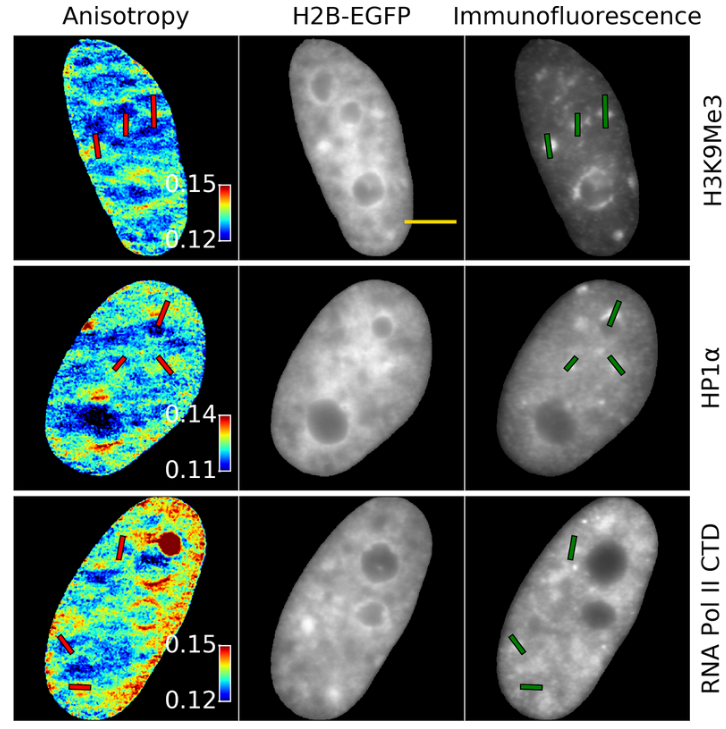
\includegraphics[trim=0 5 0 30, clip,width=0.8\linewidth]{figures/1.png}\hspace*{\fill}}
    \caption{H2B-EGFP anisotropy corresponds to known markers of heterochromatin and euchromatin. Immunofluorescence markers shown with anisotropy maps of fixed cells. HP1$\alpha$ and H3K9Me3 are known markers of heterochromatin, and phosphorylated RNA-Pol-II-CTD is a marker for active regions of transcription, where the chromatin is more open. Scale bar corresponds to 5$\mu$m.}
    {\label{fig:an_verify}}
\end{figure}

\begin{figure}[!hbtp]
    {\hfill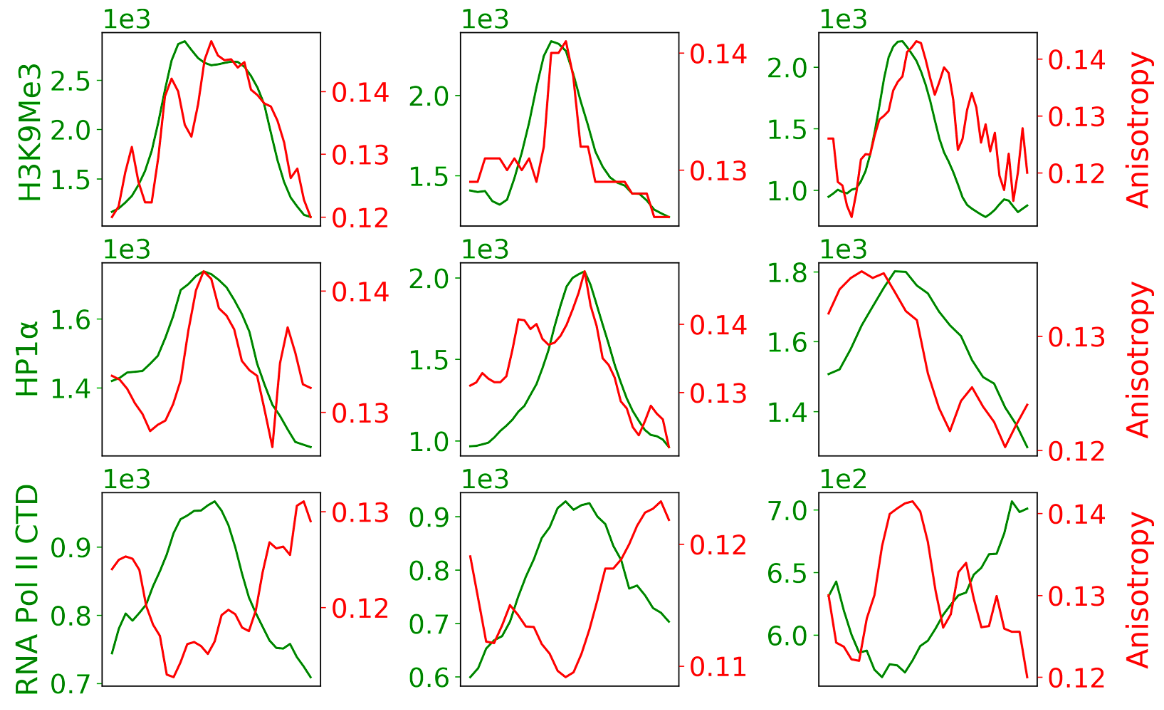
\includegraphics[clip,width=0.8\linewidth]{figures/2.png}\hspace*{\fill}}
    \caption{H2B-EGFP anisotropy corresponds to known markers of heterochromatin and euchromatin. Line profile of lines draw in the images in (Fig. \ref{fig:an_verify}) (green in immunofluorescence image, red in anisotropy map). Line profiles show that heterochromatin corresponds to regions of high anisotropy, while euchromatin corresponds to regions of low anisotropy. X-axis is distance along the line.}
    {\label{fig:an_verify_line}}
\end{figure}

\subsection{Microscopy}
\subsection{Anisotropy imaging}
\subsection{Laser microirradiation}

\subsection{Characterization}
\subsection{Image processing pipeline}

\paragraph*{} In order to verify that the anisotropy values indeed correspond to biologically relevant structures of chromatin, we first demonstrated that anisotropy maps are preserved in fixation; we then imaged HeLa cells expressing H2B-EGFP for known markers of chromatin structures with immunofluorescence assay. We found that trimethylated lysine at ninth position in core Histone H3 (H3K9Me3), which is generally associated with densely packed heterochromatin regions correspond to high values of anisotropy (Fig. \ref{fig:an_verify}, \ref{fig:an_verify_line}). Similarly, we found that Heterochromatin Protein 1$\alpha$ (HP1$\alpha$), associated with heterochromatin domains, are also enriched in regions of high anisotropy. Conversely, we stained for decompacted chromatin using an antibody against the activated form of RNA polymerase, in which S5 is phosphorylated in C-terminal domain, and found that the anisotropy values are low in such regions. Together, these results suggested that regions of high and low anisotropy indeed correspond to biologically relevant structures of dense and loosely packed chromatin.  

\begin{figure}[H]
    {\hfill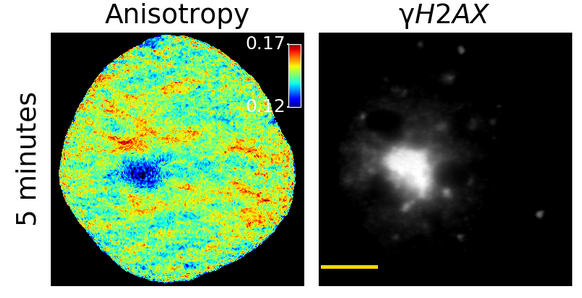
\includegraphics[clip,width=0.8\linewidth]{figures/micro_gh2ax.png}\hspace*{\fill}}
    \caption{Microirradiation activates DNA damage responses. $\gamma$H2AX, a known marker for damage response, is found at the site of microirradiation.}
    {\label{fig:micro_gh2ax}}
\end{figure}
\section{Chromatin compaction with FAI}
\subsection{Live and Fixed cell measurements}
\subsection{FAI and IF}
\subsection{Multipoint FAI}
\subsection{Analysis parameters}
\paragraph*{} We verified that microirradiation indeed causes damage by fixing and staining microirradiated cells for $\gamma$H2AX, which was observed at the site of damage (Fig. {\ref{fig:micro_gh2ax}}), indicating activated damage response.

The strength of FAI is that it allows the monitoring of chromatin compaction in living cells, but if it can be combined with fixed cell immunofluorescence, it can open up new possibilities of studying DDR on a cell- by-cell basis because of the different antibodies available against damage and chromatin markers. A previous study has shown that nucleosome level mobility is not abrogated by fixation (Hihara et al., 2012). Encouraged by this observation, we wondered whether FA maps may be preserved in fixation. This was indeed the case, and fixing HeLa cells stably expressing H2B-EGFP with 4.pc paraformaldehyde (PFA) for 15 min did not significantly alter the anisotropy maps (Supplemental Figure 1). While the anisotropy values are dimensionless fractional numbers, and the variation within the nucleus is between 0.10 and 0.19 in the nucleus shown, it should be borne in mind that this range can correspond to a change of between 18 and 215 centipoise in terms of local viscosity for a molecule such as fluorescein (Supplemental Figure 2). Given the good correspondence observed between the live-cell and fixed-cell anisotropy maps, this could potentially enable the combination of anisotropy imaging with immunostaining for different chromatin and DDR marker proteins. Thus, next, we checked the biological relevance of the anisotropy maps generated using markers for euchromatin and heterochromatin. HeLa cells expressing H2B-EGFP were fixed and stained for different heterochromatin and euchromatin markers. Correspondence of these biologically relevant chromatin compaction states with respective anisotropy maps for H2B-EGFP in the same cells was investigated. Trimethylated lysine at the ninth position in core histone protein H3 (H3K9Me3) is a histone modification that is generally associated with densely packed heterochromatin regions (Nakayama et al., 2001). Heterochromatin Protein $\alpha$ (HP$\alpha$) is associated with heterochromatin domains and is another marker for densely packed chromatin (Lachner et al., 2001). Indeed, corroborating our expectations, line profiles across regions of high levels of H3K9me3 and HP$\alpha$ showed them to be regions of high anisotropy (Figure 1). Conversely, when we stained cells for decompacted regions of active transcription, using an antibody against the activated form of RNA polymerase, in which S5 is phosphorylated in the C-terminal (Dahmus, 1996) of the largest subunit, we found the regions of stronger phospho-RNAPII staining to be anticorrelated to local anisotropy (Figure 1). We also used mouse NIH 3T3 fibroblast cells that show clear nodes of pericentric heterochromatin. NIH 3T3 cells transiently transfected with H2B-EGFP show high-contrast anisotropy maps, with pericentric heterochromatin in chromocenters corresponding to high-anisotropy regions (Supplemental Figure 3). Together, these results suggest that regions of high and low anisotropy indeed correspond to densely packed heterochromatin and loosely packed euchromatin, respectively.


The main strength of FAI is that it can report on chromatin compaction states in living cells. And because anisotropy maps are preserved in fixation, as demonstrated in the previous section, live-cell dynamics upon DNA damage can be followed by immunofluorescent detection of damage markers in the very same cells. We used FAI to study the changes to chromatin structure that has undergone microirradiation induced DSBs as employed by previous studies (Kruhlak et al., 2006; Burgess et al., 2014; Strickfaden et al., 2016). We modified our FAI microscope to introduce a 405-nm laser into the light path and used Hoechst-sensitized cells to cause local double-strand breaks of the DNA. Minutes after irradiation, strong staining for $\Gamma$H2AX and the phosphorylated form of Chk1 (p-Chk1, a target of the master DDR kinase ATR) was observed at the site of damage (Supplemental Figure 4), which indicated that the damage response was in action. Using this microirradiation protocol, we collected anisotropy data for the damaged cells over a period of 2 h, imaged once every 5 min. Anisotropy at the site of the damage could not be ascertained due to localized photobleaching of H2B-EGFP upon irradiation, but the response of the rest of the chromatin, which did not see direct irradiation, could be followed. In comparison to the control undamaged cells (N = 13), the overall $\Delta$anisotropy value ($\Delta$anisotropy = rt – r0, where rt is the mean anisotropy at any given time point, and r0 is the mean anisotropy for the 0th time point) of the irradiated cells increased with time (Figure 2B), though the response was heterogeneous among cells (Supplemental Figure 5). And though the mean rise is small, one should keep in mind that anisotropy values are themselves fractional; also, mean anisotropy averages over regions where compaction increases and surrounding regions where it decreases correspondingly, keeping the changes in mean anisotropy small. This heterogeneity is captured in the anisotropy maps, and indeed a fraction of cells show formation of nodes of high local compaction even in regions that have not directly been damaged (Figure 2A). To quantify this better and visualize the nodes, we thresholded the anisotropy map with a threshold value of “mean + 2 sigma,” where mean is the mean anisotropy value of the nucleus before damage and sigma is the SD. Values below the threshold are turned to gray, so that it becomes easier to visualize the high–anisotropy value pixels formed upon irradiation (Supplemental Figure 5C). The formation of high-anisotropy nodes is reflected in the overall increase in high-anisotropy pixels for irradiated cells as compared with control cells. However, it should be noted that the control cells also show a fair degree of heterogeneity among themselves, and this could be because of toxic effects of the imaging excitation light (Ge et al., 2013), natural cell cycle–driven processes that causes chromatin compaction changes, or systematic changes to anisotropy with photobleaching. Nonetheless, the propensity for increased compaction in irradiated cells is clear and significantly different from the dynamics of control cells. When the individual $\Delta$anisotropy time trace for each irradiated cell is examined closely (Supplemental Figure 5), 21 out of 27 cells show positive increase in delta anisotropy and only 6 out of 27 cells show an overall negative trend over the 2 h after damage, whereas in control cells, 7 out of 13 cells show a positive trend and 6 out of 13 cells show a negative trend. This indicates that there is inherent variability in the cellular response to damage, but overall there is condensation of chromatin in response to damage.

Next we wanted to combine the time course of anisotropy imaging with live-cell detection of other markers of the damage response. For this, we chose chromobody-mediated detection of early and late markers of DDR—PARP1 and PCNA. PARP1 is known to be transiently enhanced at sites of damage in response to irradiation-induced DSBs (Chou et al., 2010; Qi et al., 2019), while PCNA, being the DNA clamp, would be required for the processivity of the DNA polymerase in the final steps of repair (Moldovan et al., 2007). We independently transfected PARP1 and PCNA chromobodies tagged with TagRFP in HeLa cells stably expressing H2B-EGFP. Chromobodies (ChromoTek) are small intracellular antibodies tagged with fluorescent protein. Their major advantage is that they detect the endogenous proteins they are designed against without artifacts of overexpression of those proteins in transient transfections (Burgess et al., 2012; Panza et al., 2015). As expected, PARP1 was recruited to the site of damage almost immediately upon irradiation (Figure 3A). However, the PARP1 signal diffused away from the site by 15 min after damage, as expected (Haince et al., 2008; Mortusewicz et al., 2007). To our surprise, however, PCNA, which should be involved in the repair only at later stages, was also recruited immediately to the site of damage (Figure 3B). This was the case in G1 and G2 cells where the PCNA chromobody was homogenous in the nucleus, and even in S phase cells where the PCNA chromobody was punctated, as PCNA follows the replication fork (Supplemental Movies 1 and 2). The PCNA chromobody is primarily used for cell-cycle stage detection (Burgess et al., 2012). This implies that in response to clustered DSBs, even PCNA from replication forks is recruited to the site of damage. PCNA persisted at the site of damage for the duration of the time course, longer than PARP1 (Figure 3C). This local enrichment was quantified by plotting the mean intensity of the chromobody at the site of damage normalized to the mean intensity outside. (We found this to be a more robust metric for the enrichment, compared with just the normalized intensity at the site of damage, which decays due to photobleaching during the time course, in addition to actual dynamics. This metric is more robust because photobleaching operates both within and outside the site of damage.) But while PCNA persists longer, within 20 min, there are nodes of PCNA formed, away from the site of damage, which correspond to regions of lower anisotropy (Figure 3; Supplemental Figure 6). We asked whether these sites of PCNA enrichment and low anisotropy represent simply sites of repair factor storage or of active repair. We reasoned that if they are indeed sites of repair, even in the G1 or G2 phase, we may be able to see incorporation of a deoxynucleotide analog such as ethynyl deoxyuridine (EdU). HeLa cells transfected with the PCNA chromobody were subjected to laser-induced DSBs. G1 or G2 cells that have a homogenous distribution of the PCNA chromobody in the nucleus were chosen. We observed that at these sites of transient PCNA nodes, EdU is incorporated, which is an indication of new DNA being synthesized at these sites (Figure 3E; Supplemental Figure 7). We ruled out bleedthrough of PCNA signal in the EdU channel by imaging plates for cells with and without EdU treatment (Supplemental Figure 7). Thus, though the DSBs are induced locally, these nodes of PCNA incorporating EdU further away may indicate a looping out of individual DSBs from the site of primary damage.


Steady-state fluorescence anisotropy imaging has been used previously for measuring chromatin compaction in living cells (Banerjee et al., 2006). We established that anisotropy maps are preserved in fixation, and regions of high and low anisotropy indeed correspond to heterochromatin and euchromatin, respectively. In the context of DDR, our fluorescence anisotropy imaging studies suggest that the undamaged chromatin is globally compacted in response to localized DSB damage. In regions away from the site of damage, we observe chromatin nodes forming, as well as transient accumulation of phospho-ATM and PCNA in specific sites that correspond to more loosely packed regions of chromatin. These low-anisotropy regions with accumulated repair proteins could be regions of repair or of factors poised for repair. In future studies, we aim to investigate the possibility of blocking damage response in cells using small molecule inhibitors for DDR master kinases and what effects it has on the chromatin response upon damage. A limitation of this study is that we follow the response of undamaged chromatin because of local clustered DSBs, but anisotropy information is lost at the site of damage because of photobleaching. This could potentially be circumvented by using a histone H2B tagged with photoactivable GFP (H2B-PA-GFP). Condensation of the damaged chromatin could indeed be observed in such an experiment (Supplemental Figure 8).



\paragraph*{} In summary, we developed fluorescence anisotropy imaging to map regions of chromatin in live cells, and incorporated microirradiation to damage chromatin, and measure its dynamics post damage with live cell imaging. Following live cell imaging, we fixed the cells, and performed immunofluorescence assay against known markers of damage response to observe the state of those endogenous proteins.

\chapter{Chromatin is globally compacted upon local damage, with nodes of repair in decondensed regions}

\paragraph*{} The advantage of FAI is in the fact that it could be useful for observing chromatin dynamics in live and fixed cells. Since we have introduced a 405nm laser in our widefield setup with the dual lamp housing (Fig. {\ref{fig:setup}}), we could microirradiate specific regions in hoechst-sensitized HeLa H2B-EGFP cells, and cause a localized damage, and monitor the change in the global state of chromatin compaction. Using DNA damage markers, we can follow damage repair dynamics along with chromatin compaction states. 

\section{Microirradiation induced damage}

\begin{figure}[!htp]
    {\hfill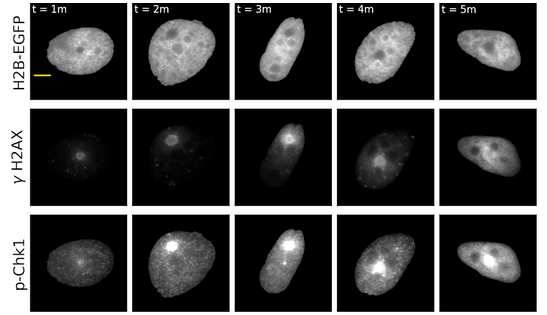
\includegraphics[clip,width=1\linewidth]{figures/pchk1.png}\hspace*{\fill}}
    \caption{Pan-nuclear induction of $\gamma$H2A.X in response to laser microirradiation. Hoechst-sensitized cells were microirradiated at intervals of 1 minute, with a different cell being irradiated every minute. Cells are fixed and stained for markers of damage response, $\gamma$H2A.X and phospho-Chk1 (a target of the ATR kinase). These are representative cells, but generally too induction of $\gamma$H2A.X is seen at the site of damage at the early timepoints, but it spreads out and there is pan-nuclear $\gamma$H2A.X induction 5-10 minutes onwards. Phospho-Chk1 is still enriched at the site of damage even at these later time-points. Scalebar is 5$\mu$m.}
    {\label{fig:chk1}}
\end{figure}


\paragraph*{} We used fluorescence anisotropy imaging to study the changes to chromatin structure that has undergone microirradiation induced DSBs as employed by previous studies \cite{kruhlak2006changes, BURGESS20141703,strickfaden2016poly}. We modified our FAI microscope to introduce a 405-nm laser into the light path and used Hoechst-sensitized cells to cause local double-strand breaks of the DNA. Minutes after irradiation, strong staining for $\gamma$H2AX and the phosphorylated form of Chk1 (p-Chk1, a target of the master DDR kinase ATR) was observed at the site of damage (Fig. {\ref{fig:chk1}}), which indicated that the damage response was in action. Using this microirradiation protocol, we collected anisotropy data for the damaged cells over a period of 2 h, imaged once every 5 min (Fig. {\ref{fig:live_an}}). Anisotropy at the site of the damage could not be ascertained due to localized photobleaching of H2B-EGFP upon irradiation, but the response of the rest of the chromatin, which did not see direct irradiation, could be followed. In comparison to the control undamaged cells (N = 13), the overall $\Delta$anisotropy value ($\Delta$anisotropy = rt – r0, where rt is the mean anisotropy at any given time point, and r0 is the mean anisotropy for the 0th time point) of the irradiated cells increased with time (Fig. {\ref{fig:timetrace}}), though the response was heterogeneous among cells ((Fig. {\ref{fig:hetero}})). And though the mean rise is small, one should keep in mind that anisotropy values are themselves fractional; also, mean anisotropy averages over regions where compaction increases and surrounding regions where it decreases correspondingly, keeping the changes in mean anisotropy small. This heterogeneity is captured in the anisotropy maps, and indeed a fraction of cells show formation of nodes of high local compaction even in regions that have not directly been damaged (Fig. {\ref{fig:live_an}}). To quantify this better and visualize the nodes, we thresholded the anisotropy map with a threshold value of “mean + 2 $\sigma$,” where mean is the mean anisotropy value of the nucleus before damage and $\sigma$ is the standard deviation of the mean. Values below the threshold are turned to gray, so that it becomes easier to visualize the high–anisotropy value pixels formed upon irradiation (Fig. {\ref{fig:thresholded}}). The formation of high-anisotropy nodes is reflected in the overall increase in high-anisotropy pixels for irradiated cells as compared with control cells. However, it should be noted that the control cells also show a fair degree of heterogeneity among themselves, and this could be because of toxic effects of the imaging excitation light, natural cell cycle–driven processes that causes chromatin compaction changes, or systematic changes to anisotropy with photobleaching. Nonetheless, the propensity for increased compaction in irradiated cells is clear and significantly different from the dynamics of control cells. When the individual $\Delta$anisotropy time trace for each irradiated cell is examined closely (Fig. {\ref{fig:closely}}), 21 out of 27 cells show positive increase in delta anisotropy and only 6 out of 27 cells show an overall negative trend over the 2 h after damage, whereas in control cells, 7 out of 13 cells show a positive trend and 6 out of 13 cells show a negative trend. This indicates that there is inherent variability in the cellular response to damage, but overall there is condensation of chromatin in response to damage.


\begin{figure}[H]
    {\hfill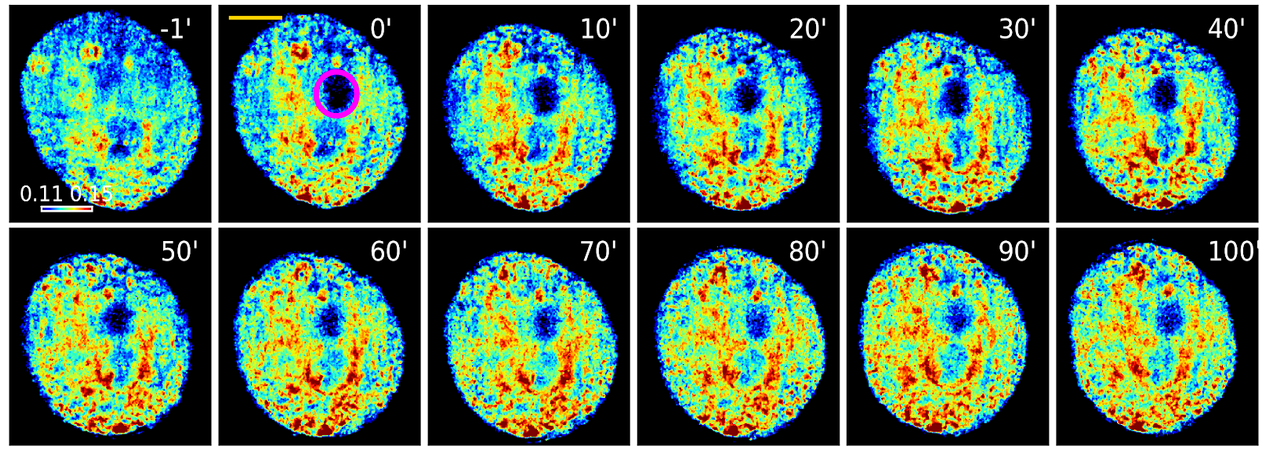
\includegraphics[clip,width=1\linewidth]{figures/live_an.png}\hspace*{\fill}}
    \caption{Dense nodes of chromatin are formed in microirradiated cells. H2B-EGFP anisotropy time series for a representative irradiated cell before and after irradiation, imaged every 5 min for over 2 h. The color map is scaled from 0.11 to 0.15. Scale bar corresponds to 5$\mu$m. Magenta circles indicate the sites of microirradiation.}
    {\label{fig:live_an}}
\end{figure}

\begin{figure}[H]
    {\hfill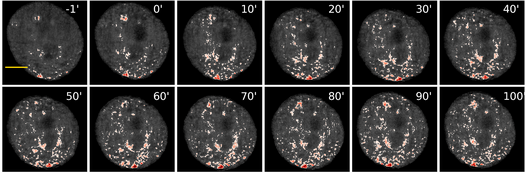
\includegraphics[clip, width=1\linewidth]{figures/thresholded.png}\hspace*{\fill}}
    \caption{A gray anisotropy map is plotted with color for anisotropy values greater than a threshold (mean + 2*standard deviation) calculated with respect to the -1' timepoint. The fraction of pixels above this constant threshold calculated for the -1' timepoint visibly grows with time indicating local compaction. Scale bar corresponds to 5$\mu$m.}
    {\label{fig:thresholded}}
\end{figure}

\begin{figure}[H]
    {\hfill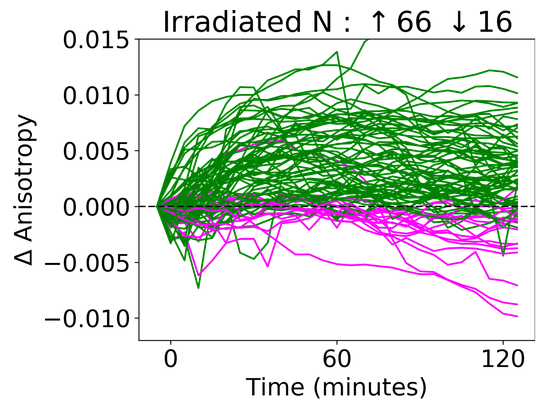
\includegraphics[clip, width=0.8\linewidth]{figures/closely.png}\hspace*{\fill}}
    \caption{Pooled single cell traces for irradiated cells done on three different days. 66 show a positive (green) trend and 16 a negative (magenta) trend.}
    {\label{fig:closely}}
\end{figure}


\paragraph*{} We microirradiated live cells and imaged them over 2 hours, every 5 minutes and computed their anisotropy maps (Fig. \ref{fig:live_an}). Since the 405nm laser bleaches EGFP locally, we could not obtain anisotropy information from the site of damage, but the anisotropy map of rest of the chromatin was unaffected. We quantified the change in anisotropy over time with $\Delta$Anisotropy, and found that as opposed to control (\(N=13\)), $\Delta$Anisotropy for irradiated cells (\(N=27\)) increased over time (Fig. \ref{fig:timetrace}). This indicated that there is increased compaction in the undamaged regions of chromatin in response to a local microirradiation. We fixed the cells after the course of imaging, and stained for common markers of DNA damage responses, and found that the phosphorylated form of DNA master kinase, ATM, forms nodes throughput the nucleus in a fraction of damaged cells (Fig. \ref{fig:patm}). These nodes are found in low anisotropy regions, indicating that these might be sites of damage repair. However, we were limited in observing the dynamics of repair factors, since fixing the cells destroys biological dynamics. In order to overcome this limitation, we utilized the chromobody technology (ChromoTek), and independently co-transfected H2B-EGFP expressing cells with chromobodies tagged with TagRFP against early and later markers of DDR, namely PARP1 and PCNA. Using this, we aimed to observe the dynamics of damage response in live cells, combined with chromatin compaction states as revealed by live anisotropy imaging.

\begin{figure}[H]
    {\hfill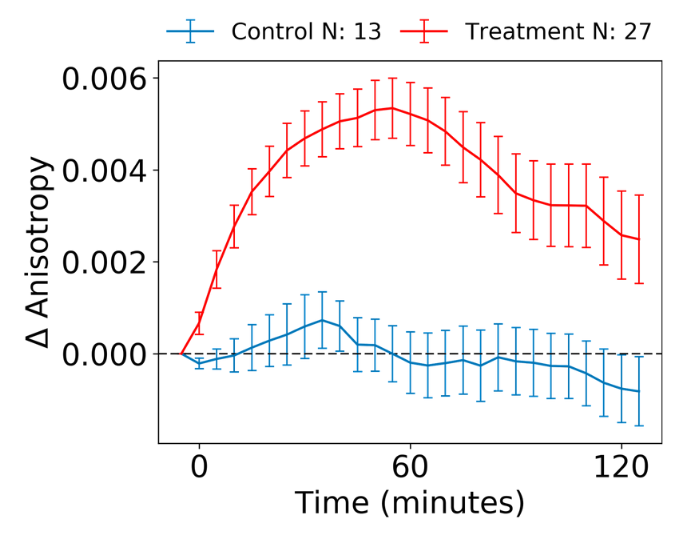
\includegraphics[clip, width=0.5\linewidth]{figures/timetrace.png}\hspace*{\fill}}
    \caption{$\Delta$Anisotropy is calculated by subtracting the mean anisotropy of any time point, with the mean anisotropy of the first time point for that cell. A positive $\Delta$Anisotropy corresponds to compaction, whereas a negative $\Delta$Anisotropy corresponds to decompaction.}
    {\label{fig:timetrace}}
\end{figure}


\begin{figure}[!htp]
    {\hfill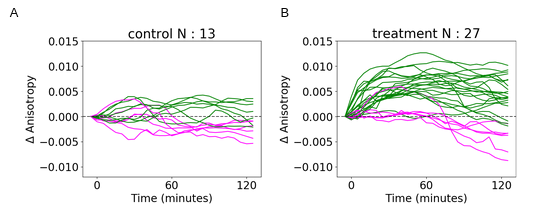
\includegraphics[clip, width=1\linewidth]{figures/hetero.png}\hspace*{\fill}}
    \caption{Compaction of undamaged chromatin in response to local damage.Individual $\Delta$anisotropy time traces of A. control (13 cells) and B. irradiated cells (27 cells). Cells with an overall positive trend are color-coded green, while those with a negative trend color-coded magenta. }
    {\label{fig:hetero}}
\end{figure}

\begin{figure}[!htp]
    {\hfill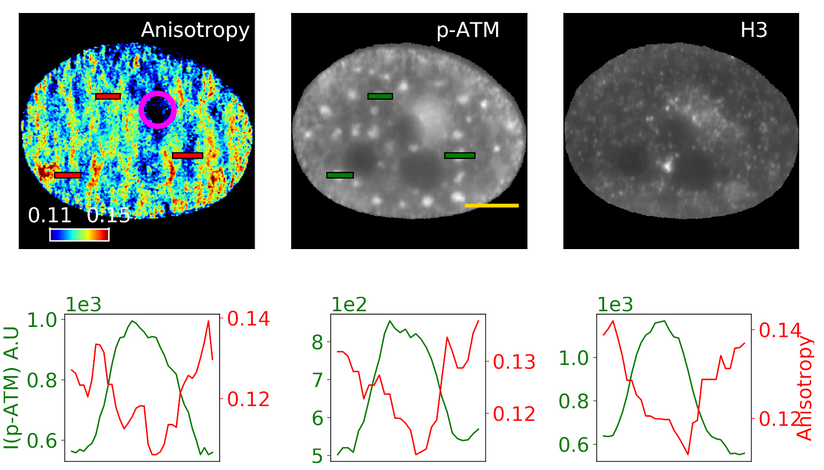
\includegraphics[clip, width=1\linewidth]{figures/patm.png}\hspace*{\fill}}
    \caption{Microirradiated cells are fixed after live imaging, and stained for damage markers. Phosphorylated-ATM is seen at sites of low anisotropy regions, and Histone H3 is accumulated at the site of damage. The purple circle is the site of microirradiation.}
    {\label{fig:patm}}
\end{figure}

\paragraph*{} PARP1 is a well characterized member of the poly (ADP ribose) polymerase (PARP) family of proteins, which are known to be transiently enhanced at sites of damage post microirradiation \cite{chou2010chromatin, qi2019multiple}. PARP1 is activated in the presence of broken DNA, which leads to the formation of poly (ADP ribose) (PAR), upon which further downstream repair factors are recruited. PCNA (proliferating cell nuclear antigen), a ring-shaped DNA replication cofactor, is a member of the family of DNA sliding clamps. It encircles DNA during replication, and enhances the processivity of DNA polymerase. PCNA is known to be associated with the final stages of DDR when new DNA has to be synthesized post excision of damaged DNA \cite{moldovan2007pcna}.

\begin{figure}[H]
    {\hfill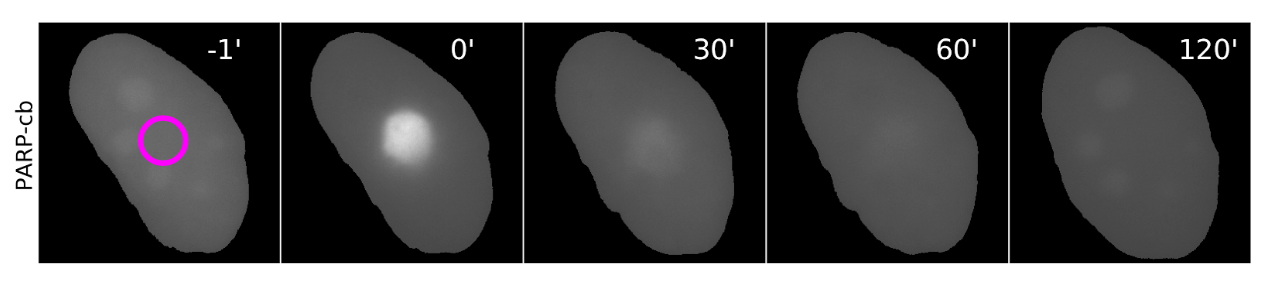
\includegraphics[clip, width=1\linewidth]{figures/parp.png}\hspace*{\fill}}
    \caption{Live cell dynamics of PARP-chrombody in irradiated cells, transiently transfected in HeLa H2B-EGFP cells. PARP1 showed immediate transient encrichment at the site of damage, and became homogenous quickly.}
    {\label{fig:parp}}
\end{figure}

\begin{figure}[H]
    {\hfill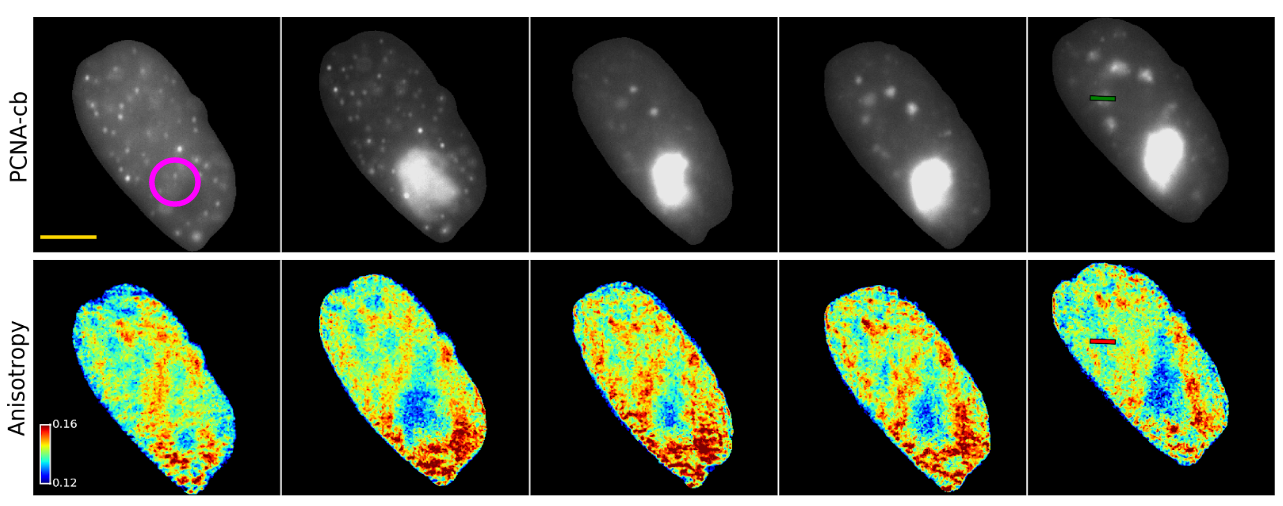
\includegraphics[clip, width=1\linewidth]{figures/pcna.png}\hspace*{\fill}}
    \caption{HeLa H2B-EGFP cells expressing PCNA chromobody along with its corresponding anisotropy maps, imaged at an  interval of 5 minutes post-irradiation. Scale bar corresponds to 5$\mu$m. Timestamps are same as (Fig. \ref{fig:parp})}
    {\label{fig:pcna}}
\end{figure}


\paragraph*{} We found that PARP1 was almost immediately recruited to site of damage upon microirradiation (Fig. \ref{fig:parp}), and diffused away from the site 15 minutes after damage. However, PCNA, which is a late stage repair protein, was also recruited immediately to the site of damage, and was found to be persistent at site of damage(Fig. \ref{fig:pcna}). We captured this behavior by quantifying the mean intensity of the chromobody at the site of damage, normalized to the mean intensity outside. (Fig. \ref{fig:retention})

\paragraph*{} While PCNA persists longer at the site of damage, within 20 minutes of irradiation, there are nodes of PCNA formed away form the site of damage. These nodes correspond to low-anisotropy regions, and incorporate EdU (ethynyl deoxyuridine), a thymidine analogue for labelling proliferating cells, suggesting that they are sites of damage repair.

\begin{figure}[H]
    {\hfill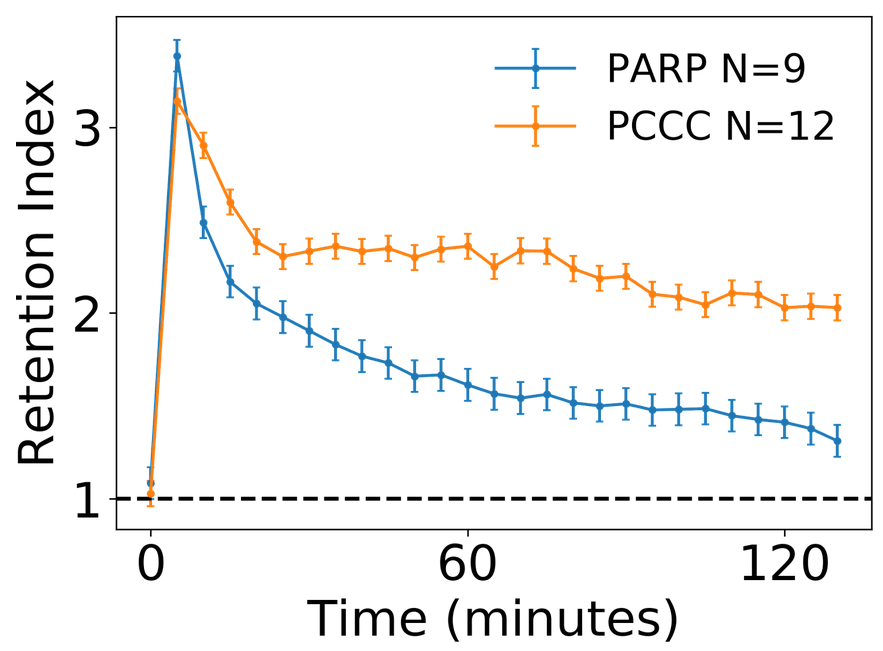
\includegraphics[clip, width=0.5\linewidth]{figures/retention.png}\hspace*{\fill}}
    \caption{PCNA persists at the site of damage longer than PARP. Retention index of any time point is defined as the ratio of intensity for a chromobody at the site of damage and outside the site of damage.}
    {\label{fig:retention}}
\end{figure}

\paragraph*{} We noticed that within 2 min after microirradiation, there is phosphorylation of Ser139 of the histone variant H2AX at the site of microirradiation, indicating DNA damage (Supplemental Figure 4). Although $\gamma$H2AX is a DNA damage marker, which is generally found as foci in regions of damaged chromatin, there is also a pan-nuclear spreading of $\gamma$H2AX in undamaged chromatin as early as 5 min after damage. In another study, interference with chromatin compaction at the damage site reduces the efficiency of damage repair. This suggested that condensation of chromatin is a necessary step in the activation of DDR (Burgess et al., 2014). However, ATM activation in mouse fibroblasts showed chromatin opening independent of DNA damage (Ji et al., 2017). During damage, ATM is thought to be activated not by direct binding to DNA strand breaks, but by changes in chromatin structure. Thus, forced compaction of chromatin promotes activation of ATR and ATM even where there are no strand breaks (Burgess et al., 2014), and conversely, activation of these kinases can change chromatin compaction (Becker et al., 2014). Thus, pan-nuclear induction of DDR (for which $\gamma$H2AX is a proxy) can drive compaction of undamaged chromatin, and the processes could feed back onto each other.

Such pan-nuclear induction of $\gamma$H2AX has been reported before when clustered DNA damage was induced by ionizing radiation, which is regulated by ATM and DNA-PK (Meyer et al., 2013). Other studies have discussed a ring of $\gamma$H2AX in the context of apoptosis (Solier and Pommier, 2014). It is possible that some of the cells we have irradiated will undergo apoptosis, and apoptotic response over and above the DNA damage response complicates the observed chromatin phenotypes. But apoptosis is accompanied by visible changes in the cell and nuclear morphology. However, our irradiated cells, under similar irradiation conditions, do not exhibit apoptotic morphology or fragmented chromatin, and many survive 48 h after irradiation. Furthermore, during the 2-h time course over which the cells were imaged, there was no significant induction of apoptotic or general cell death markers (Supplemental Figure 9). This indicates that the compaction we observe may have to do with the early processes of DDR rather than the long-term processes of cell death because of excessive DNA damage.

PCNA, surprisingly, is shown to be recruited immediately to the site of localized DSBs, independent of cell-cycle phase. As interestingly, at longer time-points it forms transient nodes of repair away from the site of damage in regions of more open chromatin (low anisotropy). These nodes actively incorporate EdU, indicating active repair and possibly a looping of DSBs from the primary laser-induced cluster to open regions of chromatin for the purposes of repair.

Our study establishes the possibility of using FAI to measure chromatin compaction changes in the context of DNA damage in living cells, followed by immunofluorescence for DDR and chromatin markers. While the response to DSBs is investigated here, following previous studies (Kruhlak et al., 2006; Burgess et al., 2014), in principle, the method is amenable to other forms of DNA damage as well, which we aim to investigate in the future.

\paragraph*{} In summary, we observed the dynamics of chromatin compaction state, and correlated it with markers of damage, such as phosphorylated ATM, which forms nodes at low anisotropy regions. We found that damage repair markers have different dynamics, as PARP1 has low retention in the site of damage, as opposed to PCNA, which persists for longer time period. We also observed that PCNA forms nodes of repair, away from the site of damage, which correspond to regions of low anisotropy and EdU incorporation.





 Next we wanted to combine the time course of anisotropy imaging with live-cell detection of other markers of the damage response. For this, we chose chromobody-mediated detection of early and late markers of DDR—PARP1 and PCNA. PARP1 is known to be transiently enhanced at sites of damage in response to irradiation-induced DSBs (Chou et al., 2010; Qi et al., 2019), while PCNA, being the DNA clamp, would be required for the processivity of the DNA polymerase in the final steps of repair (Moldovan et al., 2007). We independently transfected PARP1 and PCNA chromobodies tagged with TagRFP in HeLa cells stably expressing H2B-EGFP. Chromobodies (ChromoTek) are small intracellular antibodies tagged with fluorescent protein. Their major advantage is that they detect the endogenous proteins they are designed against without artifacts of overexpression of those proteins in transient transfections (Burgess et al., 2012; Panza et al., 2015). As expected, PARP1 was recruited to the site of damage almost immediately upon irradiation (Figure 3A). However, the PARP1 signal diffused away from the site by 15 min after damage, as expected (Haince et al., 2008; Mortusewicz et al., 2007). To our surprise, however, PCNA, which should be involved in the repair only at later stages, was also recruited immediately to the site of damage (Figure 3B). This was the case in G1 and G2 cells where the PCNA chromobody was homogenous in the nucleus, and even in S phase cells where the PCNA chromobody was punctated, as PCNA follows the replication fork (Supplemental Movies 1 and 2). The PCNA chromobody is primarily used for cell-cycle stage detection (Burgess et al., 2012). This implies that in response to clustered DSBs, even PCNA from replication forks is recruited to the site of damage. PCNA persisted at the site of damage for the duration of the time course, longer than PARP1 (Figure 3C). This local enrichment was quantified by plotting the mean intensity of the chromobody at the site of damage normalized to the mean intensity outside. (We found this to be a more robust metric for the enrichment, compared with just the normalized intensity at the site of damage, which decays due to photobleaching during the time course, in addition to actual dynamics. This metric is more robust because photobleaching operates both within and outside the site of damage.) But while PCNA persists longer, within 20 min, there are nodes of PCNA formed, away from the site of damage, which correspond to regions of lower anisotropy (Figure 3; Supplemental Figure 6). We asked whether these sites of PCNA enrichment and low anisotropy represent simply sites of repair factor storage or of active repair. We reasoned that if they are indeed sites of repair, even in the G1 or G2 phase, we may be able to see incorporation of a deoxynucleotide analog such as ethynyl deoxyuridine (EdU). HeLa cells transfected with the PCNA chromobody were subjected to laser-induced DSBs. G1 or G2 cells that have a homogenous distribution of the PCNA chromobody in the nucleus were chosen. We observed that at these sites of transient PCNA nodes, EdU is incorporated, which is an indication of new DNA being synthesized at these sites (Figure 3E; Supplemental Figure 7). We ruled out bleedthrough of PCNA signal in the EdU channel by imaging plates for cells with and without EdU treatment (Supplemental Figure 7). Thus, though the DSBs are induced locally, these nodes of PCNA incorporating EdU further away may indicate a looping out of individual DSBs from the site of primary damage.


 In the context of DDR, our fluorescence anisotropy imaging studies suggest that the undamaged chromatin is globally compacted in response to localized DSB damage. In regions away from the site of damage, we observe chromatin nodes forming, as well as transient accumulation of phospho-ATM and PCNA in specific sites that correspond to more loosely packed regions of chromatin. These low-anisotropy regions with accumulated repair proteins could be regions of repair or of factors poised for repair. In future studies, we aim to investigate the possibility of blocking damage response in cells using small molecule inhibitors for DDR master kinases and what effects it has on the chromatin response upon damage. A limitation of this study is that we follow the response of undamaged chromatin because of local clustered DSBs, but anisotropy information is lost at the site of damage because of photobleaching. This could potentially be circumvented by using a histone H2B tagged with photoactivable GFP (H2B-PA-GFP). Condensation of the damaged chromatin could indeed be observed in such an experiment (Supplemental Figure 8).

\chapter{Up-scaling experimentation in cell biology}
\paragraph*{} Existing microscope software requires a human operator to scan the sample visually, and identify regions of interest for imaging sample objects. However, it is difficult for the human user to manually comb through the sample to find fields of interest. Combing the sample for objects can also expose it to large amount of light, which can cause photobleaching of the flurophores or create destructive phototoxicity artifacts \cite{scherf2015smart}. Besides, the execution plan of the microscope is rigid, and the user must take care to configure the plan correctly, and there is no scope for error correction during an acquisition without discarding data or timepoints. Feedback of the validity of the experimental data is often obtained in the image analysis stage of the microscopy experiment, by which time it is too late to influence the experiment, take corrective measures such as reimaging the sample. Such problems are fundamental to microscopy technology, and are faced by several others in fields such as super-resolution microscopy \cite{D1SC05506B}. We developed full-stack microscopy, which combines acquisition with analysis, which is often considered separate steps of an imaging experimental workflow. This allows us to get a direct feedback of experimental quality during the course of imaging. In our case, we wanted to maximize the sample size of common DDR experiments, while minimizing light exposure to the sample prior to data acquisition.


\section{Overview of existing technology}
\paragraph*{}The software systems of commonly available widefield systems can be characterized as open loop systems. The user configures the microscope for a specific mode of operation by choosing appropriate device parameters manually. Some of these parameters are position of stage, Z drive, mirrors, shutter, detector exposure, detector gain, choice of objective, etc. Many of these parameters are optimally set to attain the best image possible by the system in order to perform further downstream analysis. The best image is often characterized as an image that has one or many or a part-of an object of interest (such as cells, tissues, crystals, etc), is well focused, well-illuminated, with good contrast, and without any over-exposed pixels, which are niquest sampled.

Some of these considerations for best image translates to the user having to manually scan the sample, which can have different forms, such as a confocal dish, slide, or a multi-well plate, in search of fields of interest. In the case of a confocal dish, one has to ensure that the field of interest is not set in the periphery of the coverslip area, where light will move through glass and plastic, reducing the quality of the image. Other considerations of the field might be determined by the object of interest under observation. One might want to image only cells transfected with a certain plasmid expressing one or more fluorescent proteins. Or one might be interested in imaging cells of certain cell cycle stage, such as mitotic or s-phase cells. In such scenarios, to identify fields of interest is a task of human persistance. The more effort one can spend in identifying fields of interest, one casts a wider net of observation on their objects of interest, therefore increasing the throughput of the experiment.

The establishment of fields of interest by manual inspection translates to a list of stage coordinates, with which the microscope executes an imaging sequence, resulting in the production of data. Existing commercial software present this model which can be characterized as an open loop, where the chain of execution is linear, and there are no feedback in the operation of the system.

The user takes the data from the microscope software, and often starts a separate control sequence for image analysis, which results in quantifiable information that can be graphically represented to support the initial hypothesis. The analysis maybe manually done with ImageJ or automated partially or fully with macros or using other programming languages capable of image processing and statistical analysis, such as Python, or Matlab. This disconnect between the control sequences of imaging and analysis creates a gap in the experimental process that has to be bridged by the human user. In case the analysis reveals problems in imaging (such as focus drift, xy-drift, over or under exposed image, or insufficient sample size), there is no way for the analysis control sequence to make adjustments to the acquisition control sequence to compensate for low-quality data. Even if such compensations are done manually, it is time-consuming and might not yield the desired experimental conditions for the user. It is analogous to the era of satellite imaging (before digital camera) which used photographic films to image the Earth, and the film had to be later ejected into the atmosphere, captured, and developed in a lab, and often the pictures were out of focus, or had cloud cover over their area of interest, marking for poor returns from a costly mission. Experiments with biological sample could be time-bound, and would have to be verified for quality at every acquisition step. Sample undergoing treatment conditions, or samples such as primary tissues are time-sensitive and cannot be imaged again once a timepoint has elapsed. Corrections would have to be performed online in case of any imaging failure. However, with the disconnect between acquisition and analysis, it is not often possible to make such corrections without manual inspection at the time of acquisition, making this a high-effort endeavour.


\section{Microscope software from scratch}
In order to combine the acquisition and analysis of microscope software, and to build on top of that, one would have to write a microscope control software from scratch. In a control system point of view, a microscope can be abstracted as a combination of motors and detectors. Motors are devices such as the filter wheel, objective turret, temperature control unit, condensor unit, etc. and detectors are the camera unit, or a quadrant photodiode that returns a reading of the sample. The challenge is to be able to communicate with these devices and be able to set and read state parameters of these motors programmatically. Such as, reading the current position configuration of the filter wheel, or setting the objective turret to new position. For any motor-like device, this can be abstracted as set and read functions.

Microscope software can be thought of as abstractions of increasing complexity that work on top of each other. At the most basic level, the microscope software should be able to send commands to the device, and receive responses. This is often known as the control layer, which facilitates control at the hardware level. In the other hand, the device receives the command signal from the user, executes it, and sends a response. This communication to the device is often facilitated through a serial communication protocol, which takes messages to and from the device through a physical medium, such as a cable with multiple pins, the two ends of which are attached to the motherboard of the control computer and the device that is to be controlled. In the computer end, there are device drivers, which organized for the specific device for the messages to be sent through the serial port, for the high level tasks that are to be accomplished for that device. For instance, there might be an exposure set command to set a certain exposure for the camera, or a snapshot command for taking a snapshot. At the device level, these might translate to a multitude of actions, which are abstracted away inside the device. The device acts as a message parsing hub, which receives messages, performs actions and replies with data.


With the control over the hardware with device drivers defined, it then becomes a matter of establishing connection with all the devices, and orchestrating the order in which the devices are asked to perform a certain task programmatically. I utilized pymmcore, the python wrapper for micro-manager to get raw access to the control layer of the microscope hardware (Olympus IX83, Andor Zyla camera) \cite{edelstein2014advanced}. This enabled me to change the state of different motors, and read image data from the camera. In order to write elaborate sequences of hardware orchestration, I integrated the micro-manager control layer with bluesky experimental framework, a spectroscopy based data acquisition framework, which gave me the necessary higher-level abstractions to define complex workflows, redundancies, error-checking and data management \cite{allan2019bluesky}.


In the bluesky framework, the devices are defined by the ophyd architecture, which are python objects which have methods to set and read data using the control layer. These objects are utilized in bluesky plans, which are higher level representation of the logic of device orchestration required for an experimental procedure. Plans are written with the help of atomic instructions, which are interpreted by a RunEngine. This architecture isolates the logic of the experimental procedure from the technical implementations of the device control instructions, while also giving access to the data generated, along with proper handling of metadata, and live visualization among other things. Examples of atomic instructions may include mv, which sets a value for a given motor, or mvr, which sets a value relative to current value, or read, which takes a reading and adds it the current bundle of readings.

To write a typical microscopy experimental pattern in bluesky, such as a Z scan, one would have to define a FocusMotor and a Camera ophyd object, with appropriate access to the control layer defined. Then, within a for loop, which defines the range of distances to cover, either in absolute or relative terms, the atomic plans of mv or mvr are called on the FocusMotor, followed by a read on the Camera on every iteration of the for loop. The end results are a series of images, which are varying in the Z axis. Similar logic can be applied to scan involving any other motor devices, such as XYStage. Interestingly, one can define the exposure of the camera also as a motor, and therefore define an exposure sweep with similar programming.


\begin{figure}[H]
    {\hfill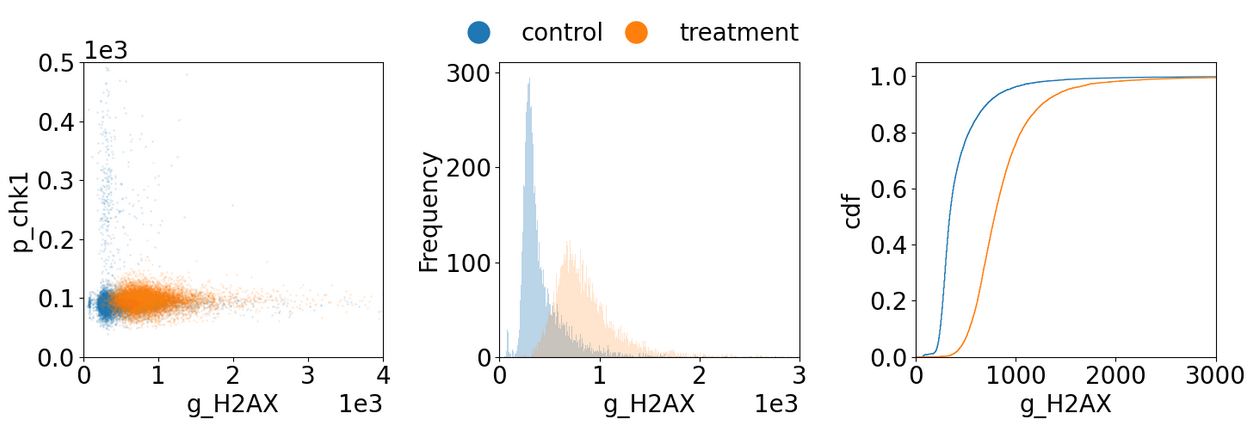
\includegraphics[clip, width=1\linewidth]{figures/ncs.png}\hspace*{\fill}}
    \caption{Automated immunofluorescence imaging against $\gamma$H2AX and phosphorylated Chk1 with a sample size of N=11000 for control and treatment each.}
    {\label{fig:ncs}}
\end{figure}

\paragraph*{} Using this tool, we pushed the limit of sample size for a damage response experiment based on immunofluorescence against $\gamma$H2AX and phosphorylated Chk1. We chemically induced damage, and imaged a total of 22000 cells, (11000 each for control and treated) with no human effort in imaging (Fig. \ref{fig:ncs}). This is far higher cell numbers than what is regularly done in microscopic investigations of DDR using everyday widefield microscopes. High Content microscopes can achieve such numbers, but we have now implemented this solution on a regular motorized widefield microscope, increasing the breadth of such investigations.

\begin{figure}[H]
    {\hfill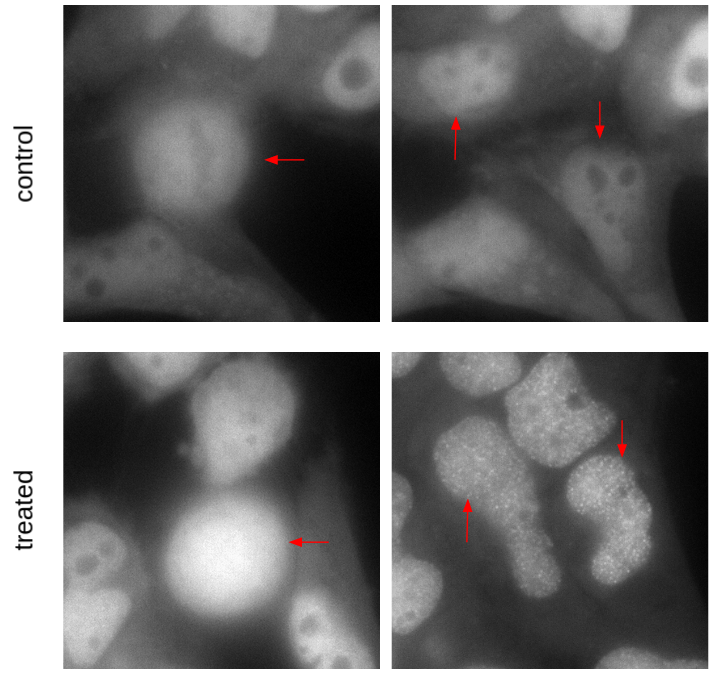
\includegraphics[clip, width=0.8\linewidth]{figures/g1.png}\hspace*{\fill}}
    \caption{G1 cells show punctated PCNA upon 4NQO damage. We followed mitotic cells (left) over time, until they divided into G1 cells. Treated G1 cells show punctated PCNA. The arrows are marking parent (left) and daughter cells (right)}
    {\label{fig:g1}}
\end{figure}

\paragraph*{} We further developed this tool to image live cells over high cell numbers to identify small subpopulations of interest. We imaged a large volume of HeLa cells expressing PCNA-chromobody, and induced damage with 4NQO. We observed that PCNA is punctated in non-S phase cells, indicating foci of repair. Furthermore, we also observed that damage foci are transferred to daughter G1 cells from a dividing mitotic cell (Fig. \ref{fig:g1}). This required us to acquire data over hundreds of cells in an asynchronous population. Potentially such studies can be done by chemically arresting cells in specific stages of the cell cycle and then releasing them. But such arrests themselves can alter measured responses, and there is value in performing studies in unperturbed asynchronous cultures.

\paragraph*{} In summary, we assembled a microscope acquisition software from scratch for hands-free high throughput data acqusition. We applied it to DDR and saw that we can push the sample size of traditional immunofluorescene experiments to N greater than 10,000 with no effort from the user. We increased throughput for live-cell imaging, and saw that PCNA foci form in bona fide G1 cells created right after a mitosis event.

\chapter{Conclusion}
In conclusion, we have enhanced the existing methods to investigate DNA damage responses in live and fixed cells. Using our tools, we have been able to damage DNA with microirradiation and observe chromatin compaction states over time. We have observed that even undamaged chromatin is compacted upon damage, and repair factors are recruited to sites of less compact chromatin, where repair processes are detected. We observed the formation of these nodes of repair, which incorporate EdU and lie in open regions of chromatin by following PCNA induction in live cells post microirradiation. These experiments led to the realization that microscopy experiments fundamentally suffer from a  problem of throughput: the lack of an advanced software, which limits their potential. Towards overcoming this challenge, we built a prototype software to run automated experiments in large scale, generating high throughput data, with higher spatio-temporal resolution. This has allowed us to capture rare events in live cells, without the need to synchronize cells with cell cycle blockers. In the days to come such tools will be critical for microscopic investigations of DDR.


\phantomsection
\addcontentsline{toc}{section}{References}
\bibliography{citations/citations}


\end{document}
